\begin{multicols}{3}
\begin{enumerate}
	\item \begin{minipage}[t]{\linewidth} Marquer en rouge l'angle alterne-interne à l'angle marqué en bleu.\\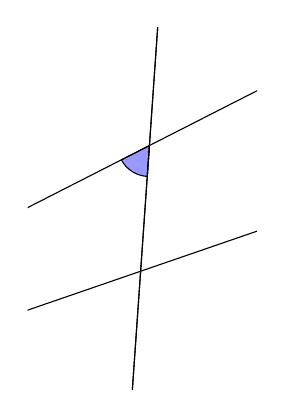
\begin{tikzpicture}[baseline,scale = 0.4]

    \tikzset{
      point/.style={
        thick,
        draw,
        cross out,
        inner sep=0pt,
        minimum width=5pt,
        minimum height=5pt,
      },
    }
    \clip (-3.7260686742862017,-5.737820251299121) rectangle (3.5625325200533546,5.737820251299121);
    	\draw  [color={black},preaction={fill,color = {blue},opacity = 0.4}] (0.06975647374412497,0.9975640502598244) -- (0.13951294748825063,1.995128100519648) -- (-0.7514935767001168,1.5411376007801016) arc (-151.86:-92.86000000000001:1) ;
	\draw[color={black}] (-44.41081326193014,-20.70439688645769)--(45.580845681095006,25.14864358723653);
	\draw[color={black}] (-3.348310739718021,-47.88307441247155)--(3.6970931084386485,52.87089466377067);
	\draw[color={black}] (-47.415441727454095,-18.273535823377483)--(48.08193440807691,14.608847776795344);
	\draw[color={black}] (-3.627336634694524,-51.87333061351086)--(3.4180672134621473,48.88063846273138);

\end{tikzpicture}\\ \end{minipage}
	\item \begin{minipage}[t]{\linewidth} Marquer en rouge l'angle alterne-interne à l'angle marqué en bleu.\\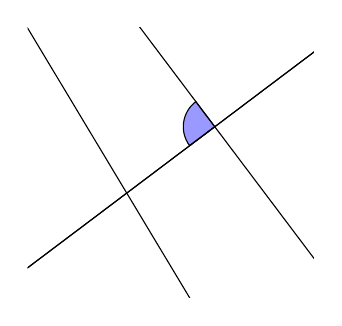
\begin{tikzpicture}[baseline,scale = 0.4]

    \tikzset{
      point/.style={
        thick,
        draw,
        cross out,
        inner sep=0pt,
        minimum width=5pt,
        minimum height=5pt,
      },
    }
    \clip (-4.343859795212818,-4.224224436834409) rectangle (4.743177550236464,4.349536576445975);
    	\draw  [color={black},preaction={fill,color = {blue},opacity = 0.4}] (0.798635510047293,0.6018150231520484) -- (1.5972710200945857,1.2036300463040968) -- (0.9954559969425373,2.0022655563513894) arc (127.02:217.01999999999998:1) ;
	\draw[color={black}] (-28.49348013750784,41.13540554866874)--(32.289837200849064,-39.52678096610784);
	\draw[color={black}] (-38.334504482270056,-28.887121111298317)--(42.32768203250652,31.896196227058557);
	\draw[color={black}] (-26.94985701057366,41.95564250037754)--(25.068988555341836,-44.6182548705358);
	\draw[color={black}] (-41.12972876743558,-30.993473692330483)--(39.532457747341,29.789843646026387);

\end{tikzpicture}\\ \end{minipage}
	\item \begin{minipage}[t]{\linewidth} Marquer en rouge l'angle correspondant à l'angle marqué en bleu.\\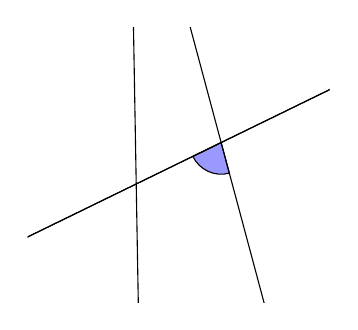
\begin{tikzpicture}[baseline,scale = 0.4]

    \tikzset{
      point/.style={
        thick,
        draw,
        cross out,
        inner sep=0pt,
        minimum width=5pt,
        minimum height=5pt,
      },
    }
    \clip (-4.794573208346252,-4.4070998056527895) rectangle (4.794573208346252,4.305334199050821);
    	\draw  [color={black},preaction={fill,color = {blue},opacity = 0.4}] (1.6070101145512712,-0.30836910610545204) -- (1.3481910694487507,0.6575567201836161) -- (0.4493970231495838,0.2191855733945388) arc (-154.32:-75.32:1) ;
	\draw[color={black}] (-11.592761185677286,48.953848034637026)--(14.547962369677307,-48.604660420558865);
	\draw[color={black}] (-43.59151124550959,-21.261000619270252)--(47.18668743070626,23.014485206426563);
	\draw[color={black}] (-2.220811391312921,49.33482803763595)--(-0.4581183411472969,-51.64978917315957);
	\draw[color={black}] (-46.287893384407106,-22.576114059637487)--(44.49030529180877,21.699371766059333);

\end{tikzpicture}\\ \end{minipage}
	\item \begin{minipage}[t]{\linewidth} Marquer en rouge l'angle correspondant à l'angle marqué en bleu.\\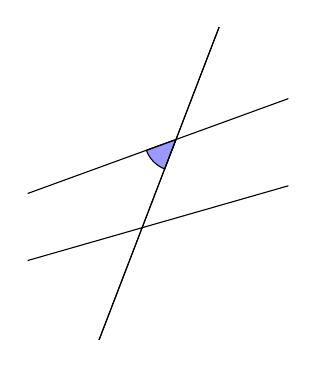
\begin{tikzpicture}[baseline,scale = 0.4]

    \tikzset{
      point/.style={
        thick,
        draw,
        cross out,
        inner sep=0pt,
        minimum width=5pt,
        minimum height=5pt,
      },
    }
    \clip (-4.171337012132907,-4.951111919237407) rectangle (4.106629786675676,4.951111919237408);
    	\draw  [color={black},preaction={fill,color = {blue},opacity = 0.4}] (0.1791839747726499,0.46679021324860104) -- (0.5375519243179505,1.4003706397458024) -- (-0.40214069646795797,1.0583504964201342) arc (-160.13:-111.13:1) ;
	\draw[color={black}] (-46.44707911497747,-15.700636526537632)--(48.46187558439928,18.843397949354905);
	\draw[color={black}] (-17.38084555294707,-45.27865068511428)--(18.814317351128267,49.012972391103084);
	\draw[color={black}] (-48.6006367212339,-15.182238430595756)--(48.48679456853631,12.657134506921151);
	\draw[color={black}] (-18.45594940158297,-48.07939196460589)--(17.739213502492365,46.21223111161149);

\end{tikzpicture}\\ \end{minipage}
	\item \begin{minipage}[t]{\linewidth} Marquer en rouge l'angle alterne-interne à l'angle marqué en bleu.\\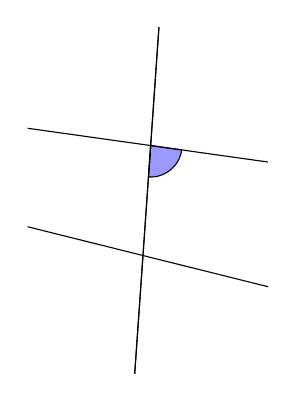
\begin{tikzpicture}[baseline,scale = 0.4]

    \tikzset{
      point/.style={
        thick,
        draw,
        cross out,
        inner sep=0pt,
        minimum width=5pt,
        minimum height=5pt,
      },
    }
    \clip (-3.800400126316241,-5.737820251299121) rectangle (3.8254389168408993,5.239038226169209);
    	\draw  [color={black},preaction={fill,color = {blue},opacity = 0.4}] (1.0949027793577586,1.357172974429671) -- (0.10463471061618787,1.4963460753897364) -- (0.03487823687206258,0.49878202512991177) arc (-93.77:-7.769999999999996:1) ;
	\draw[color={black}] (-49.40876872646233,8.455001123393007)--(50.608306216436276,-5.6014820735736);
	\draw[color={black}] (-3.3831889765900853,-48.381856437601485)--(3.662214871566587,52.372112638640786);
	\draw[color={black}] (-48.654299261288074,10.100966679463742)--(49.34556909258757,-14.333144776102706);
	\draw[color={black}] (-3.627336634694524,-51.87333061351086)--(3.4180672134621473,48.88063846273138);

\end{tikzpicture}\\ \end{minipage}
	\item \begin{minipage}[t]{\linewidth} Marquer en rouge l'angle alterne-interne à l'angle marqué en bleu.\\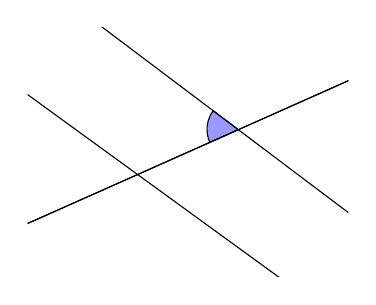
\begin{tikzpicture}[baseline,scale = 0.4]

    \tikzset{
      point/.style={
        thick,
        draw,
        cross out,
        inner sep=0pt,
        minimum width=5pt,
        minimum height=5pt,
      },
    }
    \clip (-4.860954559391704,-3.8507921867397643) rectangle (5.317727288213004,4.0525454408018);
    	\draw  [color={black},preaction={fill,color = {blue},opacity = 0.4}] (0.9135454576426014,0.4067366430758005) -- (1.827090915285202,0.8134732861516007) -- (1.0284554052379091,1.4152883093036486) arc (143.61:204.61:1) ;
	\draw[color={black}] (-38.104684587079426,30.90422444375401)--(42.557501927697125,-29.879092894602856);
	\draw[color={black}] (-43.85018196684482,-19.523358867638407)--(48.41790925505783,21.557042083017407);
	\draw[color={black}] (-41.821167905211276,28.779157650009957)--(39.889548526658416,-30.58715283152983);
	\draw[color={black}] (-47.047591068593945,-20.946937118403707)--(45.22050015330874,20.133463832252104);

\end{tikzpicture}\\ \end{minipage}
	\item \begin{minipage}[t]{\linewidth} Marquer en rouge l'angle alterne-interne à l'angle marqué en bleu.\\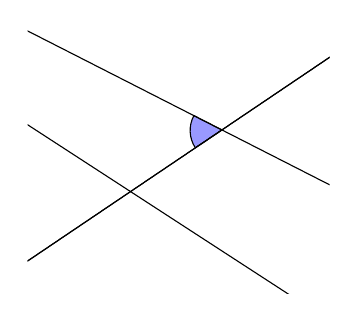
\begin{tikzpicture}[baseline,scale = 0.4]

    \tikzset{
      point/.style={
        thick,
        draw,
        cross out,
        inner sep=0pt,
        minimum width=5pt,
        minimum height=5pt,
      },
    }
    \clip (-4.509568062668835,-4.088724624415212) rectangle (5.081094717675187,4.3652149642586675);
    	\draw  [color={black},preaction={fill,color = {blue},opacity = 0.4}] (0.8290375725550416,0.5591929034707473) -- (1.658075145110083,1.1183858069414938) -- (0.7670686209217156,1.5723763066810406) arc (151.86:212.86:1) ;
	\draw[color={black}] (-42.892251064308304,23.81791079391883)--(47.09940787871684,-22.03512967977539);
	\draw[color={black}] (-39.793803482642,-26.841259366595846)--(43.93899134541721,29.63722388394958);
	\draw[color={black}] (-43.17708475610377,26.39316239554524)--(41.52864260638407,-28.61538014097251);
	\draw[color={black}] (-42.695434986584644,-28.798434528743467)--(41.03735984147456,27.680048721801974);

\end{tikzpicture}\\ \end{minipage}
	\item \begin{minipage}[t]{\linewidth} Marquer en rouge l'angle correspondant à l'angle marqué en bleu.\\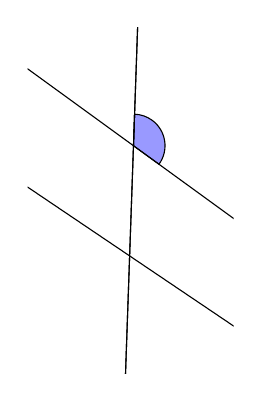
\begin{tikzpicture}[baseline,scale = 0.4]

    \tikzset{
      point/.style={
        thick,
        draw,
        cross out,
        inner sep=0pt,
        minimum width=5pt,
        minimum height=5pt,
      },
    }
    \clip (-3.2894619627188773,-5.247258721585931) rectangle (3.2468499765298446,5.7469541350954785);
    	\draw  [color={black},preaction={fill,color = {blue},opacity = 0.4}] (0.10469849010750315,2.9981724810572867) -- (0.06979899340500217,1.9987816540381913) -- (0.8788159877799495,1.4109964017457184) arc (-36.12:87.88:1) ;
	\draw[color={black}] (-40.38105072534236,31.388044268661847)--(41.329665706527315,-27.97826621287794);
	\draw[color={black}] (-1.6751758417200515,-47.970759696916595)--(1.8496733252325568,52.96771383201207);
	\draw[color={black}] (-41.504227872805835,26.460558933008706)--(42.22856695525337,-30.01792431753674);
	\draw[color={black}] (-1.7973240801788064,-51.468627591483425)--(1.7275250867738026,49.469845937445236);

\end{tikzpicture}\\ \end{minipage}
	\item \begin{minipage}[t]{\linewidth} Marquer en rouge l'angle alterne-interne à l'angle marqué en bleu.\\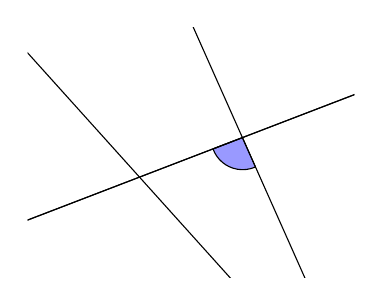
\begin{tikzpicture}[baseline,scale = 0.4]

    \tikzset{
      point/.style={
        thick,
        draw,
        cross out,
        inner sep=0pt,
        minimum width=5pt,
        minimum height=5pt,
      },
    }
    \clip (-4.951111919237408,-3.7405807889940004) rectangle (5.417902132486009,4.207372272018404);
    	\draw  [color={black},preaction={fill,color = {blue},opacity = 0.4}] (2.2738974960702034,-0.19680955855200008) -- (1.8671608529944035,0.7167358990906005) -- (0.9335804264972021,0.3583679495453004) arc (-160.13:-67.13:1) ;
	\draw[color={black}] (-18.469671300795593,46.394008781220634)--(22.610729649860197,-45.87408244068203);
	\draw[color={black}] (-44.81186047186567,-17.201661578174413)--(49.47976260435168,18.993501325900915);
	\draw[color={black}] (-34.856900957688715,36.619689349551756)--(32.72529028455597,-38.437938023665055);
	\draw[color={black}] (-48.07939196460589,-18.455949401582963)--(46.21223111161149,17.739213502492362);

\end{tikzpicture}\\ \end{minipage}
	\item \begin{minipage}[t]{\linewidth} Marquer en rouge l'angle alterne-interne à l'angle marqué en bleu.\\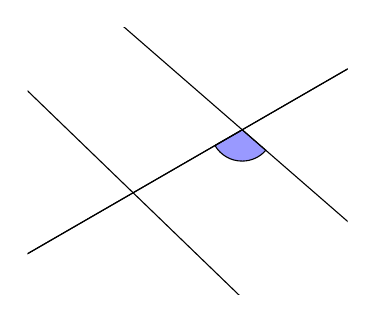
\begin{tikzpicture}[baseline,scale = 0.4]

    \tikzset{
      point/.style={
        thick,
        draw,
        cross out,
        inner sep=0pt,
        minimum width=5pt,
        minimum height=5pt,
      },
    }
    \clip (-5.080127018922193,-4.237328457790247) rectangle (5.080127018922194,4.242173537224204);
    	\draw  [color={black},preaction={fill,color = {blue},opacity = 0.4}] (2.4867603877916498,0.3439409710094923) -- (1.7320508075688776,1.0000000000000002) -- (0.8660254037844383,0.4999999999999999) arc (-149.59:-40.59:1) ;
	\draw[color={black}] (-36.00342820356974,33.80295144952537)--(40.22223939893026,-32.45901047851587);
	\draw[color={black}] (-41.56921938165308,-24.000000000000007)--(45.89934640057527,26.500000000000007);
	\draw[color={black}] (-37.69904082450143,33.73291852294986)--(34.95427900970233,-36.427576893408855);
	\draw[color={black}] (-45.03332099679081,-26)--(42.4352447854375,24.5);

\end{tikzpicture}\\ \end{minipage}
\end{enumerate}
\end{multicols}
